\section{Results}\label{sec:results}

\subsection{Static traffic in MADII's setting}\label{sec:static}
\paragraph{Reproduction check} Table~\ref{tab:repro} compares our rebuild with MADII's printed results. The headline model matches, with 19.5 rounds to FND against the paper's 19. Two of the paper's baselines that we could implement exactly, HBA and POA, land within about 15\%. One mismatch remains: our FCM matches only at later death fractions. We also ran MADII exactly as published. With the paper's $\varepsilon$ schedule ($1.0\to0.1$), training episodes collapsed to 1--1.6 rounds once exploration began, and the held-out FND was 14.9 rounds (8.2\% of the ceiling). The paper's full model size (27.3~M parameters, evaluated at episode 200 of 1{,}000) reached 15.4 rounds (8.4\%). A model 90 times larger thus lands in the same band, and the rebuild matches the paper's own figure, so MADII's shortfall is not an artefact of our implementation choices.

\begin{table}[t]
\centering
\caption{Reproduction check against MADII's printed results (30 deployments; FND in rounds).}\label{tab:repro}
\footnotesize
\begin{tabular}{@{}L{0.5\linewidth}rrr@{}}
\toprule
Method & Rebuild & Printed~\cite{yang2025madii} & Ratio\\
\midrule
MADII (Informer) & 19.5 & 19 & 1.03\\
HBA clustering & 12.4 & 14 & 0.89\\
POA clustering & 10.9 & 13 & 0.84\\
FCM clustering & 5.4 & 19 & 0.28\\
\bottomrule
\end{tabular}
\end{table}

\paragraph{Every method against the optimum} Table~\ref{tab:static} and Fig.~\ref{fig:static} give the lifetime of each method as a percentage of the LP ceiling (mean $T^*=169.7$ rounds). Battery-weighted Dijkstra keeps every node alive for 151 rounds on average, 88.4\% of the optimum, against 19.5 rounds (11.1\%) for MADII: about $8\times$ longer, with no training. It differs from min-energy Dijkstra (24.3\%) by a single factor, the battery weighting. Every one of the 30 deployments under battery Dijkstra lies between 80.8\% and 92.6\% of the optimum, whereas MADII stays between 3.9\% and 19.3\%. The gap therefore holds deployment by deployment, not only on average. LP-flow re-solved every 4 rounds reaches 94.5\%. RL warm-started from battery Dijkstra gains 0.5 points, which is not significant ($p=0.24$).

\begin{widetab}
\centering
\caption{Static traffic in MADII's setting: lifetime against the provable optimum (30 held-out deployments). W/T/L and $p$ against battery-weighted Dijkstra (Wilcoxon signed-rank).}\label{tab:static}
\footnotesize
\setlength{\tabcolsep}{4pt}
\begin{tabular}{@{}L{0.40\textwidth}rrrl@{}}
\toprule
Method & FND & \% of $T^*$ & Worst \% & W/T/L, $p$\\
\midrule
\inputtab{body/tab_static.tex}
\bottomrule
\end{tabular}
\end{widetab}

\begin{figure}[t]
\centering
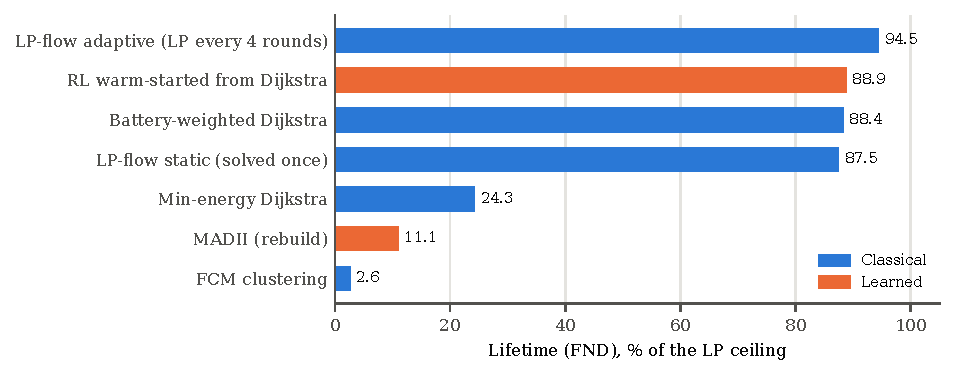
\includegraphics[width=\linewidth]{figs/static.pdf}
\caption{Static traffic in MADII's setting: mean lifetime to first node death as a percentage of the LP ceiling (30 held-out deployments).}\label{fig:static}
\end{figure}

\subsection{Time-varying traffic}\label{sec:dynamic}
Table~\ref{tab:dynamic} and Fig.~\ref{fig:ladder} report the time-varying scenarios. LEST load-table Dijkstra reaches 90.5\% of the oracle, against 85.0\% for battery-weighted Dijkstra. It wins 118 of the 120 deployments across R, N, B and D, and it gains in every scenario, including the pattern shift that nothing was tuned on (90.0\% against 83.0\%). It closes about half of the gap between battery Dijkstra and the LP planner with no solver and no training. Sharing load through the 4-tier LEST table, with its overhead charged, costs 0.3 points against exact loads (90.5\% against 90.8\%). The LP planner v2 reaches 97.0\% and beats battery Dijkstra on all 120 deployments, with a worst case of 92.1\% against 74.3\%. MADII, trained on constant traffic, stays at 13--16\%, and EBR-DA as specified at 14\%. The best of five ways of adding prediction or tuning to Dijkstra, LP-price guidance, gains 1.0 point, and the others stay at or below battery Dijkstra.

\begin{widetab}
\centering
\caption{Time-varying traffic: lifetime as a percentage of the oracle (30 held-out deployments per scenario; R: daily surge, N: constant, B: bursts, D: pattern shift). Mean $S$ weights R, N and B equally; Worst is over those 90 deployments; D is not tuned on. W/T/L against battery-weighted Dijkstra over all 120 deployments.}\label{tab:dynamic}
\footnotesize
\setlength{\tabcolsep}{4pt}\begin{tabular}{@{}L{0.33\textwidth}rrrrrrr@{}}
\toprule
Method & R & N & B & Mean $S$ & Worst & D & W/T/L\\
\midrule
\inputtab{body/tab_dynamic.tex}
\bottomrule
\end{tabular}
\end{widetab}

\begin{figure}[t]
\centering
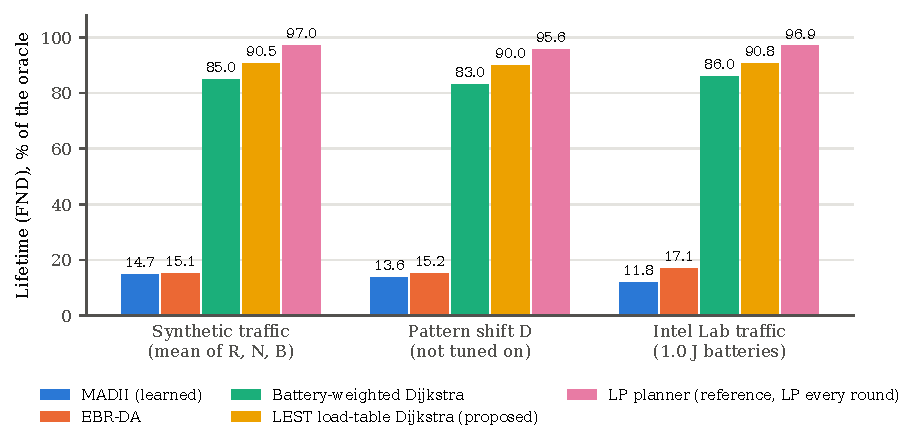
\includegraphics[width=\linewidth]{figs/ladder.pdf}
\caption{Lifetime as a percentage of the oracle on synthetic traffic, under a pattern shift and on real Intel Lab traffic.}\label{fig:ladder}
\end{figure}

\subsection{Ablation of LEST load-table Dijkstra}\label{sec:ablation}
Table~\ref{tab:ablation} removes each part of the method in turn.
\begin{itemize}[leftmargin=*]
  \item \textbf{Load only.} Without the battery weight, the load table alone reaches 45.1\%. It spreads traffic evenly but keeps relaying through nodes that are running out.
  \item \textbf{Energy only.} Without the load table the method is battery-weighted Dijkstra, at 85.0\%. It protects weak nodes but lets many nodes pile onto the same relay.
  \item \textbf{Energy in tiers.} Compressing energy into LEST tiers as well lowers validation lifetime to 43.8\% with the original trigger. A slowly draining battery never moves by more than the 0.05 band between two reports, so its tier never changes (zero tier changes in a test run). With a standard Schmitt trigger it reaches 79.2\%, and it needs 32 levels or more to recover 89\%.
  \item \textbf{Load in tiers.} The original trigger works for load: rates jump from round to round, so a tier changes in only 0.19\% of node-rounds. Finer load tables (8 or 16 levels) gain at most 0.2 points.
\end{itemize}
EBR-DA also mixes energy and load~\cite{mahdi2018ebrda}, but with a squared term that is linear in energy and over a minimum-hop tree. It reaches 15\% as specified. With its cost retuned on our bench it reaches 50.3\%, still far below the sharp $E_0/E_i$ weight combined with load booked within the round.

\begin{table}[t]
\centering
\caption{Ablation of LEST load-table Dijkstra (\% of the oracle; held-out: mean of R, N, B over 90 deployments; validation: seeds 500--511). Control bits per alive node per round in the last column.}\label{tab:ablation}
\footnotesize
\setlength{\tabcolsep}{4pt}
\begin{tabular}{@{}L{0.5\linewidth}rrr@{}}
\toprule
Variant & Held-out & Validation & Ctrl bits\\
\midrule
\textbf{Exact energy + LEST load (proposed)} & \textbf{90.5} & 90.7 & 300\\
Exact energy + exact load & 90.8 & 91.1 & 100\\
Exact energy only (battery Dijkstra) & 85.0 & 84.6 & 100\\
Load only (no battery weight) & 45.1 & 46.7 & 100\\
Exact energy + LEST load, Schmitt trigger & -- & 90.4 & 300\\
Exact energy + 8 / 16-level load & -- & 90.9 / 90.7 & 400 / 500\\
Energy also in 4 tiers, original trigger & -- & 43.8 & 400\\
Energy also in 4 tiers, Schmitt trigger & -- & 79.2 & 400\\
Energy also in 32 / 256 levels & -- & 89.0 / 89.1 & 1{,}200 / 1{,}600\\
EBR-DA as specified~\cite{mahdi2018ebrda} & 13.9 & -- & 100\\
EBR-DA cost, retuned on this bench & 50.3 & 53.3 & 100\\
\bottomrule
\end{tabular}
\end{table}

\subsection{What prediction adds}\label{sec:prediction}
\paragraph{To the LP planner} With the same v2 planner, a fixed historical rate reaches 96.5\% against 97.0\% with Holt-Winters. The difference is $+0.7$ points under surges (17/6/7, $p=0.047$ unadjusted, $p=0.19$ after Holm correction), zero with constant traffic, and not significant under bursts or the pattern shift. The forecast's clearest benefit is the worst case (92.1\% against 84.8\%). Holt-Winters already matches a perfect forecast (96.9\%), so a better forecaster could not add more. The gain comes from the planner: moving from v1 (every 4 rounds) to v2 (every round) adds 6.6, 1.1, 7.8 and 7.7 points in R, N, B and D. Re-solving from measured batteries corrects a wrong rate through the batteries themselves. What matters is a rate averaged over a full day. A reactive LP that plans with the last 4 rounds' traffic collapses to 50--53\% under surges, and persistence to 13\%.

\paragraph{To Dijkstra} Prediction, lifetime weighting, exponent tuning and LP prices all stay within about $\pm1$ point of battery Dijkstra (Table~\ref{tab:dynamic}). Stronger battery exponents are worse: $\alpha=2$, 5, 20 and 50 give 77.4\% down to 10.7\% on validation. LP prices fed back every round collapsed to 6--18\% on validation. A tracing study explains predictive Dijkstra's loss under surges. One hour before each surge, the 20\% of nodes with the highest forecast are exactly the hotspot nodes in every deployment, so the forecast senses the pattern correctly. Predictive Dijkstra does move relay traffic off those nodes before the surge (from 30.2\% to 28.2\% of relayed packets). Once the surge starts, however, the reserve vanishes, the spared nodes look rich, their relay share rises (43.6\% to 46.8\%), and a hotspot node dies first in 67\% of deployments against 47\%. Battery Dijkstra already charges every relay its energy per packet divided by its battery. Any further per-node signal moves whole subtrees onto neighbours, which then die first. LEST Dijkstra avoids this because its booking is incremental within the round.

\subsection{Real traffic: Intel Berkeley Lab}\label{sec:intel}
Table~\ref{tab:intel} shows that the ranking found on synthetic traffic holds on real traffic. At $E_0=1.0$~J, LEST Dijkstra reaches 90.8\% against 86.0\% for battery Dijkstra (16/7/4), and the LP planner reaches 96.9\%. EBR-DA reaches 17.1\% and MADII 11.8\%. The forecast is far more accurate than the historical mean here (next-day rate error 0.52 against 1.03 packets per mote-hour), yet the lifetime difference is only 0.3 points, and its visible benefit is again the worst case (88.8\% against 79.9\%). At $E_0=1.5$~J, about half the deployments outlive the dataset and count as ties, so the 1.0~J run is the cleaner comparison.

\begin{widetab}
\centering
\caption{Intel Lab traffic: lifetime as a percentage of the oracle (27 test deployments). W/T/L against battery-weighted Dijkstra.}\label{tab:intel}
\footnotesize
\setlength{\tabcolsep}{4pt}\begin{tabular}{@{}L{0.36\textwidth}rrrrrr@{}}
\toprule
& \multicolumn{3}{c}{$E_0=1.0$~J} & \multicolumn{3}{c}{$E_0=1.5$~J}\\
\cmidrule(lr){2-4}\cmidrule(l){5-7}
Method & Mean & Worst & W/T/L & Mean & Worst & W/T/L\\
\midrule
\inputtab{body/tab_intel.tex}
\bottomrule
\end{tabular}
\end{widetab}

\subsection{Statistical tests}\label{sec:stats}
Table~\ref{tab:wilcoxon} reports the paired Wilcoxon signed-rank tests for the main comparisons, and Fig.~\ref{fig:paired} shows the deployment-by-deployment pairs behind the central one.
\begin{itemize}[leftmargin=*]
  \item \textbf{LEST Dijkstra against battery Dijkstra.} LEST Dijkstra is better on time-varying traffic (median $+4.6$ points, $p_{\mathrm{Holm}}=2.2\times10^{-20}$, $r=+1.00$) and on Intel Lab traffic (median $+0.5$, $p_{\mathrm{Holm}}=0.005$, $r=+0.81$).
  \item \textbf{LP planner against LEST Dijkstra.} The LP planner is better again in both settings.
  \item \textbf{LEST against exact loads.} The 4-tier table loses a small but significant 0.5 points against exact loads on synthetic traffic ($p=6.4\times10^{-4}$), the price of sharing load in 2 bits.
  \item \textbf{Prediction and learning on Dijkstra.} Predictive Dijkstra is significantly \emph{worse} than battery Dijkstra on synthetic traffic ($p=0.007$). RL warm-started from Dijkstra is not significantly different from it ($p=0.24$).
\end{itemize}
Every adjusted $p$ for MADII and EBR-DA is below $10^{-6}$, with $r=-1$.

\begin{widetab}
\centering
\caption{Paired Wilcoxon signed-rank tests (two-sided). Mean and median are the paired differences, first method minus second, in points of the oracle percentage. Holm adjustment is applied within each setting's family of comparisons; $r$ is the matched-pairs rank-biserial correlation.}\label{tab:wilcoxon}
\footnotesize
\setlength{\tabcolsep}{4pt}\begin{tabular}{@{}L{0.30\textwidth}rrrrrr@{}}
\toprule
Comparison & Mean & Median & W/T/L & $p$ & $p_{\mathrm{Holm}}$ & $r$\\
\midrule
\inputtab{body/tab_wilcoxon.tex}
\bottomrule
\end{tabular}
\end{widetab}

\begin{figure}[t]
\centering
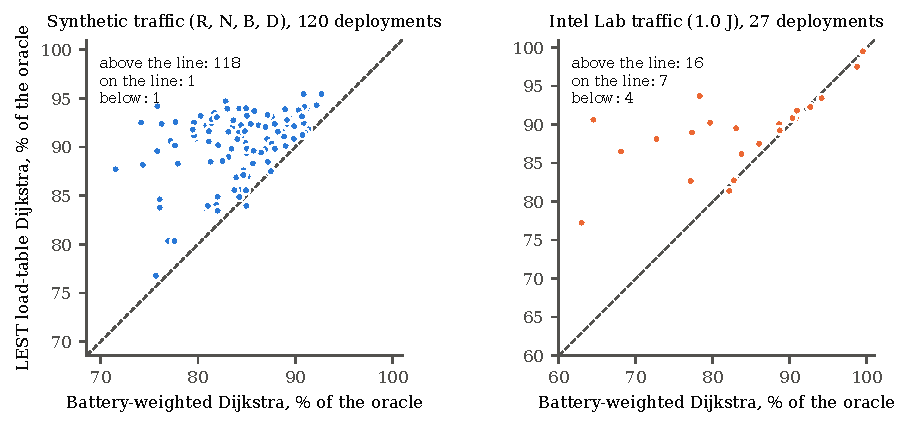
\includegraphics[width=\linewidth]{figs/paired.pdf}
\caption{Deployment-by-deployment lifetime of LEST load-table Dijkstra against battery-weighted Dijkstra. Points above the dashed line are deployments where LEST Dijkstra lives longer.}\label{fig:paired}
\end{figure}

\subsection{Traffic metrics and computation}\label{sec:computation}
Lifetime is not bought at the expense of delivery (Table~\ref{tab:traffic}). In MADII's static setting, the delivery ratio is about 99\% for every router. LEST Dijkstra delivers more data by the time half the nodes are dead (HND) than battery Dijkstra, and more per joule. MADII delivers 2.7 times less data by HND and about half as much per joule. Its one advantage is shorter paths (2.61 hops), obtained from long direct links that drain batteries. Our rebuild delivers 25{,}349~kbit by HND against the paper's printed 25{,}708, a further check on the reproduction. In computation, battery Dijkstra needs under 1~ms per round, LEST Dijkstra about 25~ms and the LP planner about 0.2~s, all at the mains-powered sink, while MADII needs 1{,}000 training episodes before use (Table~\ref{tab:characteristics}).

\begin{table}[t]
\centering
\caption{Traffic metrics in MADII's setting (constant traffic, 30 deployments). HND: rounds until half the nodes are dead. This run uses the time-varying simulator with constant traffic. The classical routers give the same FND as in Table~\ref{tab:static}, but the MADII rebuild gives 27.3 rounds rather than 19.5. Either value is below 17\% of the ceiling.}\label{tab:traffic}
\footnotesize
\setlength{\tabcolsep}{3pt}
\begin{tabular}{@{}L{0.3\linewidth}rrrrrr@{}}
\toprule
Router & FND & HND & kbit by HND & kbit/J & Deliv. & Hops\\
\midrule
LP planner v2 & 167.7 & 170.7 & 67{,}475 & 1{,}355 & 99.1\% & 3.23\\
\textbf{LEST Dijkstra} & 157.8 & 163.7 & 64{,}686 & 1{,}306 & 99.1\% & 3.34\\
Battery Dijkstra & 151.4 & 162.9 & 63{,}843 & 1{,}286 & 98.9\% & 3.53\\
Min-energy Dijkstra & 42.5 & 159.1 & 55{,}735 & 1{,}336 & 99.3\% & 3.96\\
MADII rebuild & 27.3 & 73.3 & 25{,}349 & 681 & 99.2\% & 2.61\\
MADII, printed~\cite{yang2025madii} & 19 & 89 & 25{,}708 & -- & -- & --\\
\bottomrule
\end{tabular}
\end{table}
